%!TEX root = ../main.tex
\chapter{Pandas --- Data Analysis}
\label{ch:pandas}

\begin{intuition}
Imagine a spreadsheet like Excel, but driven entirely by Python code.
That is exactly what \textbf{Pandas}\index{Pandas} offers: a powerful library
for loading, exploring, filtering, and analyzing tabular data.
In science, most experimental data come in tabular form
--- Pandas is the ideal tool to manipulate them.
\end{intuition}

% ----------------------------------------------------------------
\section{Series and DataFrames}
\index{Series}\index{DataFrame}

Pandas relies on two fundamental structures:

\begin{definition}[Series and DataFrame]
A \textbf{Series} is a labeled column of data (like a vector with an index).
A \textbf{DataFrame} is a two-dimensional table composed of several Series
sharing the same index.
\end{definition}

\begin{center}
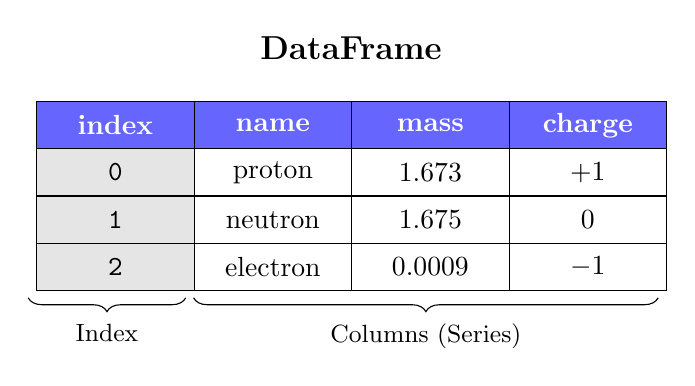
\begin{tikzpicture}[
  cell/.style={draw, minimum width=2cm, minimum height=0.6cm, anchor=north west},
  header/.style={cell, fill=blue!60, text=white, font=\bfseries},
  indexcell/.style={cell, fill=gray!20, font=\ttfamily},
]
  % Headers
  \node[header] at (0,0) {index};
  \node[header] at (2,0) {name};
  \node[header] at (4,0) {mass};
  \node[header] at (6,0) {charge};
  % Row 0
  \node[indexcell] at (0,-0.6) {0};
  \node[cell] at (2,-0.6) {proton};
  \node[cell] at (4,-0.6) {1.673};
  \node[cell] at (6,-0.6) {+1};
  % Row 1
  \node[indexcell] at (0,-1.2) {1};
  \node[cell] at (2,-1.2) {neutron};
  \node[cell] at (4,-1.2) {1.675};
  \node[cell] at (6,-1.2) {0};
  % Row 2
  \node[indexcell] at (0,-1.8) {2};
  \node[cell] at (2,-1.8) {electron};
  \node[cell] at (4,-1.8) {0.0009};
  \node[cell] at (6,-1.8) {$-1$};
  % Labels
  \draw[decorate, decoration={brace, amplitude=5pt, mirror}] (-0.1,-2.5) -- (1.9,-2.5)
    node[midway, below=6pt, font=\small] {Index};
  \draw[decorate, decoration={brace, amplitude=5pt, mirror}] (2.0,-2.5) -- (7.9,-2.5)
    node[midway, below=6pt, font=\small] {Columns (Series)};
  \node[above, font=\large\bfseries] at (4,0.4) {DataFrame};
\end{tikzpicture}
\end{center}

\begin{codeblock}[title=\textbf{Python}]
\begin{minted}{python}
import pandas as pd

# Create a Series
masses = pd.Series([1.673, 1.675, 0.0009],
                   index=["proton", "neutron", "electron"])
print(masses)
\end{minted}
\end{codeblock}

\begin{codeoutput}
\begin{verbatim}
proton      1.6730
neutron     1.6750
electron    0.0009
dtype: float64
\end{verbatim}
\end{codeoutput}

% ----------------------------------------------------------------
\section{Loading data: \py{pd.read\_csv}}
\index{read\_csv}

In practice, we rarely enter data by hand. Pandas can read many
formats: CSV, Excel, JSON, SQL, etc. We will use the
\texttt{tips}\index{tips (dataset)} dataset available in Seaborn.

\begin{codeblock}[title=\textbf{Python}]
\begin{minted}{python}
import seaborn as sns

tips = sns.load_dataset("tips")
print(type(tips))
print(tips.shape)
\end{minted}
\end{codeblock}

\begin{codeoutput}
\begin{verbatim}
<class 'pandas.core.frame.DataFrame'>
(244, 7)
\end{verbatim}
\end{codeoutput}

The DataFrame \py{tips} contains 244 rows (observations) and 7 columns.

% ----------------------------------------------------------------
\section{Quick exploration}
\index{head}\index{info}\index{describe}\index{shape}

\begin{codeblock}[title=\textbf{Python}]
\begin{minted}{python}
# First rows
print(tips.head(3))
\end{minted}
\end{codeblock}

\begin{codeoutput}
\begin{verbatim}
   total_bill   tip     sex smoker  day    time  size
0       16.99  1.01  Female     No  Sun  Dinner     2
1       10.34  1.66    Male     No  Sun  Dinner     3
2       21.01  3.50    Male     No  Sun  Dinner     3
\end{verbatim}
\end{codeoutput}

\begin{codeblock}[title=\textbf{Python}]
\begin{minted}{python}
# Statistical summary
print(tips.describe().round(2))
\end{minted}
\end{codeblock}

\begin{codeoutput}
\begin{verbatim}
       total_bill     tip    size
count      244.00  244.00  244.00
mean        19.79    3.00    2.57
std          8.90    1.38    0.95
min          3.07    1.00    1.00
25%         13.35    2.00    2.00
50%         17.80    2.90    2.00
75%         24.13    3.56    3.00
max         50.81   10.00    6.00
\end{verbatim}
\end{codeoutput}

\begin{codeblock}[title=\textbf{Python}]
\begin{minted}{python}
tips.info()
\end{minted}
\end{codeblock}

\begin{codeoutput}
\begin{verbatim}
<class 'pandas.core.frame.DataFrame'>
RangeIndex: 244 entries, 0 to 243
Data columns (total 7 columns):
 #   Column      Non-Null Count  Dtype
---  ------      --------------  -----
 0   total_bill  244 non-null    float64
 1   tip         244 non-null    float64
 2   sex         244 non-null    category
 3   smoker      244 non-null    category
 4   day         244 non-null    category
 5   time        244 non-null    category
 6   size        244 non-null    int64
\end{verbatim}
\end{codeoutput}

% ----------------------------------------------------------------
\section{Selecting data}
\index{loc}\index{iloc}

\begin{definition}[loc vs iloc]
\py{loc} selects by \textbf{labels} (row/column names).
\py{iloc} selects by \textbf{integer positions} (numeric indices).
\end{definition}

\begin{codeblock}[title=\textbf{Python}]
\begin{minted}{python}
# Select a column
print(tips["total_bill"].head(3))

# Select by position (row 0, column 1)
print(tips.iloc[0, 1])      # 1.01

# Select by label
print(tips.loc[0, "tip"])    # 1.01

# Multiple columns
subset = tips[["total_bill", "tip"]].head(3)
print(subset)
\end{minted}
\end{codeblock}

\begin{codeoutput}
\begin{verbatim}
0    16.99
1    10.34
2    21.01
Name: total_bill, dtype: float64
1.01
1.01
   total_bill   tip
0       16.99  1.01
1       10.34  1.66
2       21.01  3.50
\end{verbatim}
\end{codeoutput}

% ----------------------------------------------------------------
\section{Filtering with Boolean masks}
\index{Boolean mask}\index{filtering}

\begin{codeblock}[title=\textbf{Python}]
\begin{minted}{python}
# Bills greater than 40
large_meals = tips[tips["total_bill"] > 40]
print(large_meals[["total_bill", "tip", "size"]])
\end{minted}
\end{codeblock}

\begin{codeoutput}
\begin{verbatim}
     total_bill   tip  size
11        35.26  5.00     4
23        39.42  7.58     4
39        31.27  5.00     3
47        32.40  6.00     4
56        38.01  3.00     1
59        48.27  6.73     4
170       50.81  10.00    3
182       45.35  3.50     3
197       43.11  5.00     4
212       48.33  9.00     4
\end{verbatim}
\end{codeoutput}

\begin{codeblock}[title=\textbf{Python}]
\begin{minted}{python}
# Multiple conditions: Sunday dinners with tip > 5
filtered = tips[(tips["day"] == "Sun") & (tips["tip"] > 5)]
print(f"Number of results: {len(filtered)}")
print(filtered[["total_bill", "tip", "day"]].head())
\end{minted}
\end{codeblock}

\begin{codeoutput}
\begin{verbatim}
Number of results: 11
     total_bill    tip  day
23        39.42   7.58  Sun
39        31.27   5.00  Sun
44        30.40   5.60  Sun
47        32.40   6.00  Sun
52        34.81   5.20  Sun
\end{verbatim}
\end{codeoutput}

% ----------------------------------------------------------------
\section{Aggregation with GroupBy}
\index{groupby}\index{aggregation}

The \py{groupby} operation groups data by a categorical variable,
then applies an aggregation function.

\begin{codeblock}[title=\textbf{Python}]
\begin{minted}{python}
# Average tip per day
per_day = tips.groupby("day")["tip"].mean().round(2)
print(per_day)
\end{minted}
\end{codeblock}

\begin{codeoutput}
\begin{verbatim}
day
Thur    2.77
Fri     2.73
Sat     2.99
Sun     3.26
Name: tip, dtype: float64
\end{verbatim}
\end{codeoutput}

\begin{codeblock}[title=\textbf{Python}]
\begin{minted}{python}
# Multiple statistics
stats = tips.groupby("sex")[["total_bill", "tip"]].agg(["mean", "std"])
print(stats.round(2))
\end{minted}
\end{codeblock}

\begin{codeoutput}
\begin{verbatim}
       total_bill        tip
             mean   std mean  std
sex
Male        20.74  9.25 3.09 1.49
Female      18.06  8.01 2.83 1.16
\end{verbatim}
\end{codeoutput}

% ----------------------------------------------------------------
\section{Quick visualization with \py{df.plot()}}
\index{plot (Pandas)}

Pandas integrates matplotlib to create plots in a single line.

\begin{codeblock}[title=\textbf{Python}]
\begin{minted}{python}
import matplotlib.pyplot as plt

# Histogram of total bills
tips["total_bill"].plot(kind="hist", bins=20, edgecolor="black",
                        title="Distribution of total bills")
plt.xlabel("Total bill")
plt.ylabel("Frequency")
plt.show()

# Average tip per day (bar chart)
tips.groupby("day")["tip"].mean().plot(kind="bar", color="blue",
                                        title="Average tip per day")
plt.ylabel("Average tip")
plt.show()
\end{minted}
\end{codeblock}

\begin{codeblock}[title=\textbf{Python}]
\begin{minted}{python}
# Scatter plot: total bill vs tip
tips.plot(kind="scatter", x="total_bill", y="tip", alpha=0.6,
          title="Tip as a function of total bill")
plt.xlabel("Total bill")
plt.ylabel("Tip")
plt.show()
\end{minted}
\end{codeblock}

\begin{remark}
For more elaborate visualizations, one can use Seaborn or Matplotlib
directly. The \py{df.plot()} method is ideal for quick exploration.
\end{remark}

% ----------------------------------------------------------------
\section{Creating new columns}

\begin{codeblock}[title=\textbf{Python}]
\begin{minted}{python}
# Compute the tip percentage
tips["tip_pct"] = (tips["tip"] / tips["total_bill"] * 100).round(1)
print(tips[["total_bill", "tip", "tip_pct"]].head(4))
\end{minted}
\end{codeblock}

\begin{codeoutput}
\begin{verbatim}
   total_bill   tip  tip_pct
0       16.99  1.01      5.9
1       10.34  1.66     16.1
2       21.01  3.50     16.7
3       23.68  3.31     14.0
\end{verbatim}
\end{codeoutput}

% ----------------------------------------------------------------
\begin{errmark}{Common errors with Pandas}
\begin{enumerate}
  \item \textbf{SettingWithCopyWarning}\index{SettingWithCopyWarning} --- When modifying
    a "slice" of a DataFrame, Pandas does not know whether you are modifying the original
    or a copy. Solution: use \py{.loc[]} or \py{.copy()} explicitly.
\begin{minted}{python}
# BAD: may trigger a warning
subset = tips[tips["day"] == "Sun"]
subset["tip_pct"] = subset["tip"] / subset["total_bill"]

# GOOD: explicit copy
subset = tips[tips["day"] == "Sun"].copy()
subset["tip_pct"] = subset["tip"] / subset["total_bill"]
\end{minted}
  \item \textbf{Confusing \py{loc} and \py{iloc}} --- \py{loc[1]} accesses the row
    whose \textbf{label} is 1; \py{iloc[1]} accesses the \textbf{second} row
    (position 1). After filtering, labels are no longer consecutive!
  \item \textbf{Forgetting parentheses in multiple conditions} ---
    Write \py{(cond1) \& (cond2)}, not \py{cond1 \& cond2}.
\end{enumerate}
\end{errmark}

% ----------------------------------------------------------------
\begin{projet}{Analyzing the Tips dataset}
\begin{enumerate}
  \item Load the \texttt{tips} dataset with Seaborn.
  \item Compute the average tip by meal time (\py{time}).
  \item Determine which day has the highest number of customers (sum of \py{size}).
  \item Create a column \py{price\_per\_person} = \py{total\_bill / size}.
  \item Plot a histogram of \py{price\_per\_person} and comment on the distribution.
  \item Test whether smokers leave a different tip (groupby + mean).
\end{enumerate}
\end{projet}

% ----------------------------------------------------------------
\section{Exercises}

\begin{exercise}[$\star$]
Load the dataset \py{sns.load\_dataset("penguins")}. Display the first 5 rows,
the shape of the DataFrame, and the statistical summary. How many missing values
are there per column? (Hint: \py{.isna().sum()})
\end{exercise}

\begin{exercise}[$\star$]
From the \texttt{tips} dataset, select all rows where the total bill
exceeds 30 and the tip is less than 3. How many rows do you get?
\end{exercise}

\begin{exercise}[$\star\star$]
Use \py{groupby} to compute the mean and standard deviation of the tip
by sex \emph{and} meal time (groupby on two columns).
Which category leaves the highest average tip?
\end{exercise}

\begin{exercise}[$\star\star$]
Create a new column \py{tip\_category} that equals \py{"generous"} if
\py{tip\_pct > 20}, \py{"normal"} if between 10 and 20, and \py{"low"} otherwise.
Use \py{pd.cut} or \py{np.where}. Plot a bar chart of the number
of meals per category.
\end{exercise}

\begin{exercise}[$\star\star\star$]
Load the dataset \py{sns.load\_dataset("planets")}. Analyze the distribution of
exoplanet discovery methods over the years: group by
\py{method} and \py{year}, count the discoveries, and plot the temporal evolution
for the 3 most frequent methods.
\end{exercise}

% ----------------------------------------------------------------
\begin{keyformulas}{Chapter 8 --- Pandas: the essentials}
\begin{tabular}{@{}p{5cm} p{9cm}@{}}
\toprule
\textbf{Operation} & \textbf{Syntax} \\
\midrule
Load a CSV & \py{pd.read\_csv("file.csv")} \\
First rows & \py{df.head(n)} \\
Dimensions & \py{df.shape} \\
Statistical summary & \py{df.describe()} \\
Column selection & \py{df["col"]} or \py{df.col} \\
Selection by position & \py{df.iloc[row, column]} \\
Selection by label & \py{df.loc[row, "column"]} \\
Filtering & \py{df[df["col"] > value]} \\
Aggregation & \py{df.groupby("col")["val"].mean()} \\
New column & \py{df["new"] = expression} \\
Quick plot & \py{df.plot(kind="hist")} \\
\bottomrule
\end{tabular}
\end{keyformulas}
